\documentclass[preprint]{aastex}

% ----- Packages (kept from your source) -----
\usepackage{graphicx}
\usepackage{color}
\usepackage{yfonts}
\usepackage{pifont}
\usepackage{amsmath,amssymb,amsfonts}
\usepackage{multirow}
\usepackage{subfigure}
\usepackage{epstopdf}
\usepackage{amsthm}
\usepackage{mathtools}
\usepackage{hyperref}
\usepackage{bbm}
% ----- Custom Commands -----
\newcommand{\ans}{\textcolor{blue}{$\Rightarrow$\,\,}}
\newcommand{\iid}{{ i.i.d.\,\,}}
\newcommand{\noi}{\stackrel{\textstyle n}{\stackrel{\textstyle \rightarrow}{\infty}}}




% ----- Theorem Environments -----
\newtheoremstyle{nonitalicname}
  {}{}                 % space above/below
  {\itshape}           % body font
  {}                   % indent
  {\bfseries}          % theorem head font
  {.}                   % punctuation after theorem head (we handle it manually)
  { }                  % spacing after theorem head
  {\thmname{#1}\ \thmnumber{#2}: \thmnote{#3}}
  
\theoremstyle{nonitalicname}
\newtheorem{theorem}{Theorem}[section]
\newtheorem{lemma}[theorem]{Lemma}
\newtheorem{proposition}[theorem]{Proposition}
\newtheorem{corollary}[theorem]{Corollary}

% Definitions and theorems both italic
\theoremstyle{plain}
\newtheorem{definition}{Definition}[section]


\theoremstyle{remark}
\newtheorem{remark}{Remark}
\newcommand{\bthmref}[1]{\textbf{Theorem~\ref{#1}}}
\newcommand{\bdefref}[1]{\textbf{Definition~\ref{#1}}}
\newcommand{\blemref}[1]{\textbf{Lemma~\ref{#1}}}



% ----- Optional quality-of-life helpers -----
% Set a default graphics path (edit folder name as needed)
\graphicspath{{figures/}}

% Metadata 
\newcommand{\papertitle}{Spectral Density Estimation for Stationary Processes: AR(p) Density Approximation and Nonparametric Smoothing}
\newcommand{\paperauthor}{Summer Le}
\newcommand{\paperaffil}{Department of Statistics and Applied Probability\\
University of California, Santa Barbara\\
Santa Barbara, CA 93117}
\newcommand{\paperemail}{sle@ucsb.edu}

% ----- Document -----
\begin{document}

% ----- Title & Author -----
\title{\papertitle}
\author{\paperauthor}
\affil{\paperaffil}
\email{\paperemail}

% ----- Abstract -----
\begin{abstract}
Macroeconomic time series often exhibit macroeconomic cycles, seasonal patterns, and persistent long-run trends mixed with short-term fluctuations that are highly relevant for economic analysis and policy making. These components are often difficult to identify in the time domain, but the frequency domain provides a clearer representation by separating variance across different scales and highlighting persistent cycles, dominant or weak structural frequencies, and other systematic patterns that may not be visually apparent in the raw series. Consequently, accurate estimation of the spectral density for a stationary process is essential. In this paper, we examine two distinct methodologies for spectral estimation: a nonparametric approach based on windowed periodograms and a parametric approach grounded in ARMA model representations. Our simulation studies validate both approaches and demonstrate that parametric method excels under correct model specification while nonparametric method provides flexibility through data--driven estimation, making it particularly valuable when theoretical models are unavailable or uncertain.
\end{abstract}


% =========================
% 1. INTRODUCTION
% =========================
\section{Introduction}
% Motivate the question, cite key literature, and clearly state contributions/hypotheses.
A substantial literature on spectral density estimation has been developed, spanning both nonparametric and parametric approaches. 
The nonparametric approach to estimating spectral density offers several advantages, one of which is the flexibility since it does not require a specific model. Therefore, it is well suited for uncovering the underlying dependence pattern, which allows us to study the latent cycles, seasonal components, and other structural frequencies that may not be captured by low--order parametric models. However, these benefits come with important limitations. The periodogram is not a consistent estimator, its variance does not vanish asymptotically, which motivates the use of smoothing, tapering, or averaging procedures such as Welch’s method (\cite{welch1967}) to obtain a stable estimate. Another approach in the nonparametric realm is smoothing of the log periodogram, as demonstrated in \cite{wahba}. The log spectral density is obtained by applying a smoothing spline on the log of the periodogram, with the smoothing parameter $\lambda$ as well as the degree of the smoothing spline chosen to minimize the estimate of the integrated mean squared error. Recent advances in smoothing periodogram include Bayesian nonparametric approaches, such as in \cite{choudetal}. This paper explores constructing the prior using Bernstein polynomial, and updating the pseudoposterior distribution using Whittle likelihood, which results in consistent pseudoposterior distribution. 

The parametric approach, typically based on ARMA models, provides a convenient and analytically tractable framework for spectral estimation. Because the spectral density of an ARMA process admits a closed-form expression, computation is straightforward and statistically efficient when the model appropriately reflects the underlying dynamics. Parametric estimators generally exhibit lower variance than their nonparametric counterparts and can perform well even with relatively short samples. Beyond ARMA models, several other parametric frameworks have been developed for spectral analysis. \cite{granger} introduced the ARFIMA model by generalizing the concept of differencing to fractional orders, showing that allowing the differencing parameter $d$ to take non--integer values produces a stationary process with a parametric spectral density that decays as a power law at low frequencies, thereby capturing long--memory behavior that finite-order ARMA models cannot represent. \cite{harvey} extend the structural time-series framework by developing a state-space model in which the implied spectral density corresponds to a Butterworth--type bandpass filter. By estimating the model parameters via maximum likelihood in state--space form, the resulting Kalman smoother extracts business--cycle components through a model-implied parametric filter.

This report is organized as follows. Section 1 explores the parametric approach to spectral density estimation. We begin by establishing a theoretical result that demonstrates that the spectral density of any stationary process can be arbitrarily closely approximated by an AR($p$) spectral density under appropriate regularity conditions. This approximation approach is then assessed through simulation studies that examine both the goodness--of--fit of correctly specified models and the consequences of model misspecification. Section 2 addresses nonparametric spectral density estimation techniques, discussing computational methods leveraging circulant matrix structures and Welch's method for smoothing estimator, with the latter evaluated through simulation studies. Section 3 compiles our findings from both parametric and nonparametric frameworks, highlights the fundamental trade--offs between efficiency and robustness in spectral density estimation, and outlines promising directions for future research.
% =========================
% 3. METHODS
% =========================


\section{Spectral Density Estimation: Parametric Approach}
\subsection{Spectral Density Approximation Using AR(p) Processes}

A central idea in the parametric approach to spectral density estimation is to approximate the underlying stationary process by a member of a parametric family whose spectral density admits a closed--form expression. Among the most widely used families are autoregressive (AR) models, which allows for transparent analysis and straightforward estimation.
 

\begin{definition}
A stochastic process $\{X_t\}$ is said to be \textbf{weakly stationary or wide sense stationary (wss)} if:
$$\begin{aligned}
(a)\;& \mathbb{E}[X_t] = \mu,\\
(b)\;& \mathrm{Var}(X_t) = \sigma^2,\\
(c)\;& \gamma_X(t,s) = \gamma_X(t-s).
\end{aligned}$$
\end{definition}

Weak stationarity ensures that the second--order structure is time-invariant and that a spectral density exists.

\begin{definition}
An \textbf{autoregressive process of order $p$}, denoted AR($p$), is a stochastic process $\{Y_t\}$ satisfying
$$Y_t = \phi_1Y_{t-1}+ ... + \phi_p X_{t-p} + Z_t $$ 
where $Z_t \sim \text{WN}(0, \sigma^2)$ for all $t,s \in T$
\end{definition}
Let $\phi(z) = 1 - \phi_1 z - \cdots - \phi_p z^p$ denote the characteristic AR polynomial.  
If all roots of $\phi(z)$ lie outside the unit circle, then the AR($p$) process is causal, weakly stationary, and possesses a spectral density that can be derived as a special case of the ARMA($p,q$) result below.

\begin{theorem}[Spectral Density of the ARMA(p,q) Process]\label{thm:spectralarma}
Let $\{Y_t\}$ be an ARMA($p,q$) process, not necessarily causal or invertible, satisfying 
\begin{equation}
    \phi(B)Y_t = \theta(B)\varepsilon_t, \quad \varepsilon_t \sim \text{WN}(0, \sigma^2)
\end{equation}
where the characteristic AR and MA polynomials $\phi(\zeta)$ and $\theta(\zeta)$ 
have no common zeros, and $\phi(\zeta)$ has no zeros on the unit circle.  
Then $\{Y_t\}$ has spectral density
\begin{equation}
    f_Y(\lambda) = \frac{\sigma^2}{2\pi}
\frac{|\theta(e^{-i\lambda})|^2}{|\phi(e^{-i\lambda})|^2}, 
\quad \lambda \in [-\pi, \pi].
\end{equation}
\end{theorem}

Applying Theorem~\ref{thm:spectralarma} to the AR($p$) case (i.e., setting $\theta(e^{-i\lambda}) \equiv 1$), the spectral density of an AR($p$) process is

\begin{equation} \label{eq:ar_spectral_density}
\begin{aligned}
f_p(\lambda) &= \frac{\sigma^2}{2\pi} |\phi(e^{-i\lambda})|^{-2}\\
&= \sigma^2 (2\pi)^{-1} |\phi(e^{-i\lambda})|^{-2}\\
&= A^{-1}|\phi(e^{-i\lambda})|^{-2}
\end{aligned}
\end{equation}

where $\phi(e^{-i\lambda})
= 1 - \phi_1 e^{-i\lambda}
    - ...
    - \phi_p e^{-ip\lambda}.$, $A \triangleq 2\pi \sigma^{-2}$.

\begin{theorem}[Trigonometric Weierstrass Approximation]\label{lem:weierstrass}
Suppose $f$ is a continuous real-valued function defined on the real interval $[a,b]$. For every $\epsilon >0$  , there exists a polynomial $p$ such that for all x in $[a,b]$, we have the supremum norm $||f(x)-p(x)|| < \epsilon$
\end{theorem}

\begin{theorem}[Fej\'er--Riesz Factorization]\label{lem:fejer}
If $T_N(\lambda)=\sum_{k=-N}^{N}c_k e^{ik\lambda}$ is a nonnegative
trigonometric polynomial, then there exist $C>0$ and a polynomial
$Q(z)=\sum_{j=0}^M q_j z^j$ such that 
$$T_N(\lambda)=C\,|Q(e^{-i\lambda})|^2,\qquad \lambda\in[-\pi,\pi].$$
\end{theorem}

\begin{theorem}[Spectral Approximation]
For any stationary process with continuous spectral density $f$, the spectral density can be approximated arbitrarily well by that of a causal AR($p$) process. That is, for any $\varepsilon > 0$ there exists $p$ such that:
$$\sup_{\lambda} |f(\lambda) - f_p(\lambda)| < \varepsilon.$$
\end{theorem}
\begin{proof}
In Eqn.~\ref{eq:ar_spectral_density}, the AR(p) spectral density is $A^{-1}|\phi(e^{-i\lambda})|^{-2}$, and in order to approximate a stationary process $\{X_t\}$, we will show that there exists a small $\epsilon >0$ such that
\begin{equation}
    \mid[A|\phi(e^{-i\lambda})|^2]^{-1} - f(\lambda) \mid < \epsilon \quad \forall \lambda \in [-\pi, \pi]
\end{equation}


\begin{equation}\label{eq:ar_prox_1}
\begin{aligned}
\big| [A|\phi(e^{-i\lambda})|^2]^{-1} - f(\lambda) \big|
&= \big| [A|\phi(e^{-i\lambda})|^2]^{-1} - f_p(\lambda) + f_p(\lambda) - f(\lambda) \big| \\
&\leq \big| [A|\phi(e^{-i\lambda})|^2]^{-1} - f_p(\lambda) \big|
   + \big| f_p(\lambda) - f(\lambda) \big|.\,
   \end{aligned}
\end{equation}

where $f_p(\lambda) = \max\!\left(\frac{\epsilon}{2}, f(\lambda) \right)$, since we will be approximating the reciprocal of $f_p(\lambda)$, this choice of $f_p(\lambda)$ ensures that its reciprocal will not blow up when it gets too small. We then have:
\begin{equation}\label{eq:n}
0 \leq \big| f_p(\lambda) - f(\lambda) \big| \leq \frac{\epsilon}{2}.
\end{equation}


Let $M \triangleq \sup_{\lambda} f_p(\lambda)$, then we have the inequality: 
\begin{equation}\label{eq:fq_inequal}
    \frac{\epsilon}{2} < f_p(\lambda) < M\\
\iff \frac{1}{M} < \frac{1}{f_p(\lambda)} < \frac{2}{\epsilon}.
\end{equation}

$f(\lambda)$ is positive and symmetric $f(\lambda) = f(-\lambda)$ on the interval $[-\pi, \pi]$, hence $f_p(\lambda)$ is also positive and symmetric on $[-\pi, \pi]$, $\frac{1}{f_p({\lambda})}$ is also positive and symmetric on a compact interval, therefore we can apply Theorem \ref{lem:weierstrass}, so there exists a polynomial $P_m(cos(\lambda)) = \sum_{k=0}^N c_k cos(k\lambda)$ such that:

\begin{equation}\label{eq:pm_def}
\left|P_m(cos(\lambda)) - \frac{1}{f_p(\lambda)}\right| < \delta, \quad \text{where } \delta = \min \left( \frac{1}{2M}, \frac{\epsilon}{4M^2} \right). 
\end{equation}
In the Appdendix, we derive a suitable $\delta$. 
Next, using Euler's formula, we can rewrite our polynomial $P_m(cos(\lambda))$:
\begin{equation}\label{eq:weis}
\begin{aligned}
    P_m(cos(\lambda)) &= \sum_{k=0}^N c_k cos(k\lambda)\\
    &= \sum_{k=0}^N c_k \frac{e^{ik \lambda}+e^{-ik \lambda}}{2}\\
    &= \sum_{k=0}^N c_k \frac{e^{ik \lambda}}{2} + \sum_{k=0}^N c_k \frac{e^{-ik \lambda}}{2} \\
    &=  \sum_{k=0}^N c_k \frac{e^{ik \lambda}}{2} + \sum_{k=-N}^0 c_{-k} \frac{e^{ik \lambda}}{2} \\
    &=  \sum_{k=1}^N c_k \frac{e^{ik \lambda}}{2} + \sum_{k=-N}^{-1} c_{k} \frac{e^{ik \lambda}}{2} + c_0\\
    \text{Let } d_0 = c_0, d_k = \frac{c_k}{2}\\
    & = \sum_{k=-N}^N d_k e^{ik \lambda} \triangleq g(\lambda);\\
\end{aligned} 
\end{equation}

Substitute the result in  Eqn.~\ref{eq:weis} into  Eqn.~\ref{eq:pm_def}, we have: 
\begin{equation}\label{eq: pm_ine}
    \left|g(\lambda) - \frac{1}{f_p(\lambda)}\right| < \delta
\end{equation}

\begin{equation}
    \begin{aligned}
        g(\lambda) &\geq \frac{1}{f_p(\lambda)} - \delta \\
        \delta & \leq \frac{1}{2M} \leq \frac{1}{2 f_p(\lambda)} (\text{ follows from equation } (\ref{eq:fq_inequal}))\\
        \implies g(\lambda) & \geq \frac{1}{f_p(\lambda)} - \frac{1}{2 f_p(\lambda)} \geq 0.
    \end{aligned}
\end{equation}

Therefore, we can apply Theorem \ref{lem:fejer} to the non-negative and symmetric trigonometric polynomial $g(\lambda)$, and we can find $\phi(e^{-i \lambda}) = 1+ \phi_1e^{-i \lambda} + ...+ \phi_p e^{-i \lambda p}$ such that $g(\lambda) = A|\phi(e^{-i \lambda})|^2$. Substituting this result into Eqn.~\ref{eq: pm_ine}, we have:

\begin{equation}\label{eq:ar_prox_2}
\left| [A|\phi(e^{-i\lambda})|^2] - \tfrac{1}{f_p(\lambda)} \right| \leq \delta,
\end{equation}

Let  $k(\lambda) \triangleq \tfrac{1}{f_p(\lambda)}$ and we have $g(\lambda) = [A|\phi(e^{-i\lambda})|^2]$, then   Eqn.~\ref{eq:ar_prox_2} becomes
\begin{equation}\label{eq:xy}
    |g(\lambda)-k(\lambda)| \leq \delta
\end{equation}

We then have:
\begin{equation}\label{eq:ar_prox_3}
\begin{aligned}
\big| [A|\phi(e^{-i\lambda})|^2]^{-1} - f_p(\lambda) \big|  & = \left| \frac{1}{g(\lambda)} - \frac{1}{k(\lambda)}\right|\\
&= \left| \frac{k(\lambda)-g(\lambda)}{g(\lambda)k(\lambda)} \right|\\
&\leq \frac{\delta}{|g(\lambda)k(\lambda)|}
\end{aligned}
\end{equation}

From Eqn.~\ref{eq:xy}, we have
\begin{equation}
\begin{aligned}
    |g(\lambda) - k(\lambda)| &\leq \delta \\
    \implies g(\lambda) &\geq k(\lambda) - \delta \\
                        &= \frac{1}{f_p(\lambda)} - \delta \\
                        &\geq \frac{1}{M} - \delta \\
                        &\geq \frac{1}{2M},
\end{aligned}
\end{equation}
since 
\[
\delta = \min\!\left( \frac{1}{2M}, \frac{\epsilon}{4M^2} \right).
\]

Since $g(\lambda) \geq 0$ and $k(\lambda) = \frac{1}{f_p(\lambda)} > 0$, we obtain
\begin{equation}\label{eq:xy_bound}
|g(\lambda)k(\lambda)| 
= g(\lambda)k(\lambda) 
> \frac{1}{2M} \times \frac{1}{M} 
= \frac{1}{2M^2}.
\end{equation}

Substituting this result into Eqn.~\ref{eq:ar_prox_3} gives
\begin{equation}\label{eq:m}
\begin{aligned}
    \big| [A|\phi(e^{-i\lambda})|^2]^{-1} - f_p(\lambda) \big|
    &\leq 2M^2 \delta \\
    &\leq \frac{\epsilon}{2}.
\end{aligned}
\end{equation}

Combining Eqn.~\ref{eq:n} and Eqn.~\ref{eq:m}, we obtain 

\begin{equation}
\mid[A|\phi(e^{-i\lambda})|^2]^{-1} - f(\lambda) \mid \leq \frac{\epsilon}{2 } +  \frac{\epsilon}{2 } = \epsilon
\end{equation}


This completes our proof. 
\end{proof}

\subsection{Simulation Study: ARMA-Based Spectral Approximation of a Stationary Process}

To illustrate the connection between the spectral approximation theorem and practical model fitting, we simulate data from a known AR(2) process and then apply a standard Box–Jenkins method to determine the model applicable to this data.

The sample ACF and PACF in Figure~\ref{fig:bc_acf} indicates clear evidence of an autoregressive structure: the PACF exhibits two statistically significant spikes before cutting off, while the ACF displays a gradually decaying pattern. This behavior is consistent with an AR(2) model, therefore we move forward with using this model to approximate the spectral density.

\begin{figure}[ht!]
    \centering
    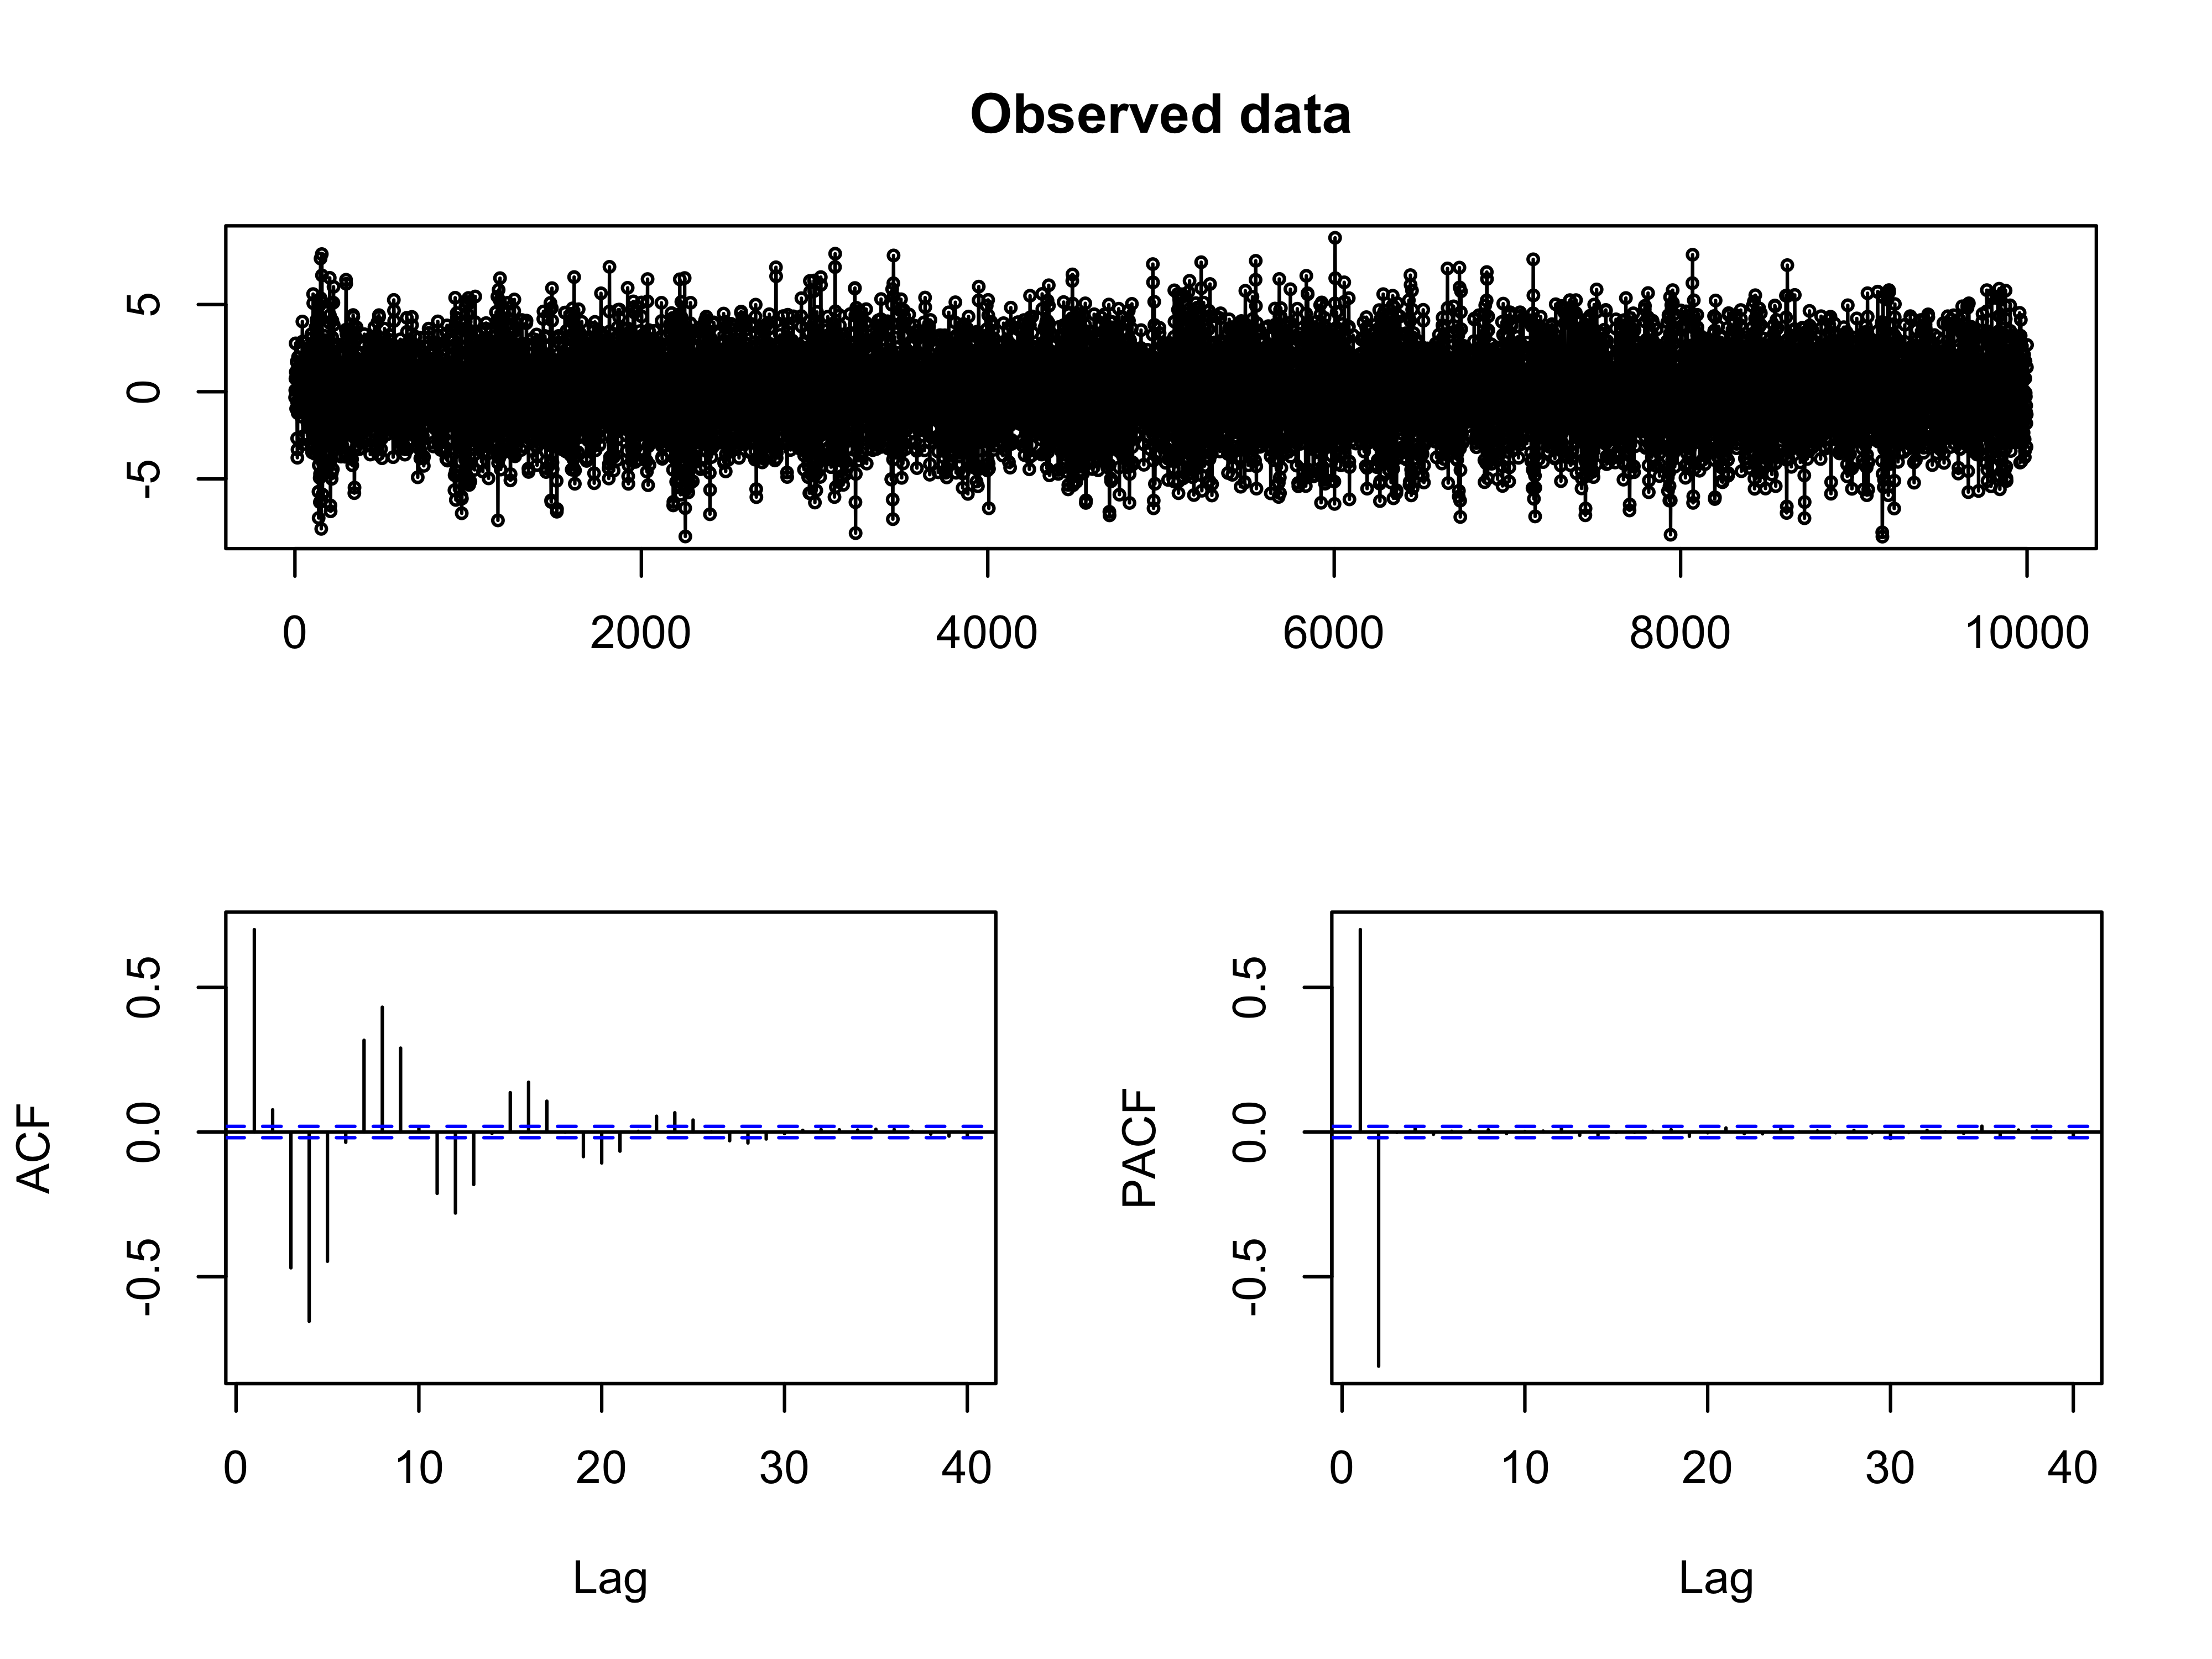
\includegraphics[width=0.8\linewidth]{tsdisplay_sim_x.png}
    \caption{\textbf{ACF and PACF of the simulated series.} The simulated series are stationary, with exponential decay in ACF and two statistically significant spikes in PACF plot, which allows us to fit an AR(2) model to this series.}
    \label{fig:bc_acf}
\end{figure}

Using the Yule-Walker equations, we obtain the estimated coefficients $\hat \phi_1 = 1.266028$ and $\hat \phi_2 = -0.8091923$. Using the formulation in  Eqn.~\ref{eq:ar_spectral_density}, we obtain the estimated spectral density $\widehat F_p(\lambda)$ for the AR(2) model, which can be observed from Figure~\ref{fig:ar2_vs_true}. 

\begin{figure}[ht!]
    \centering
    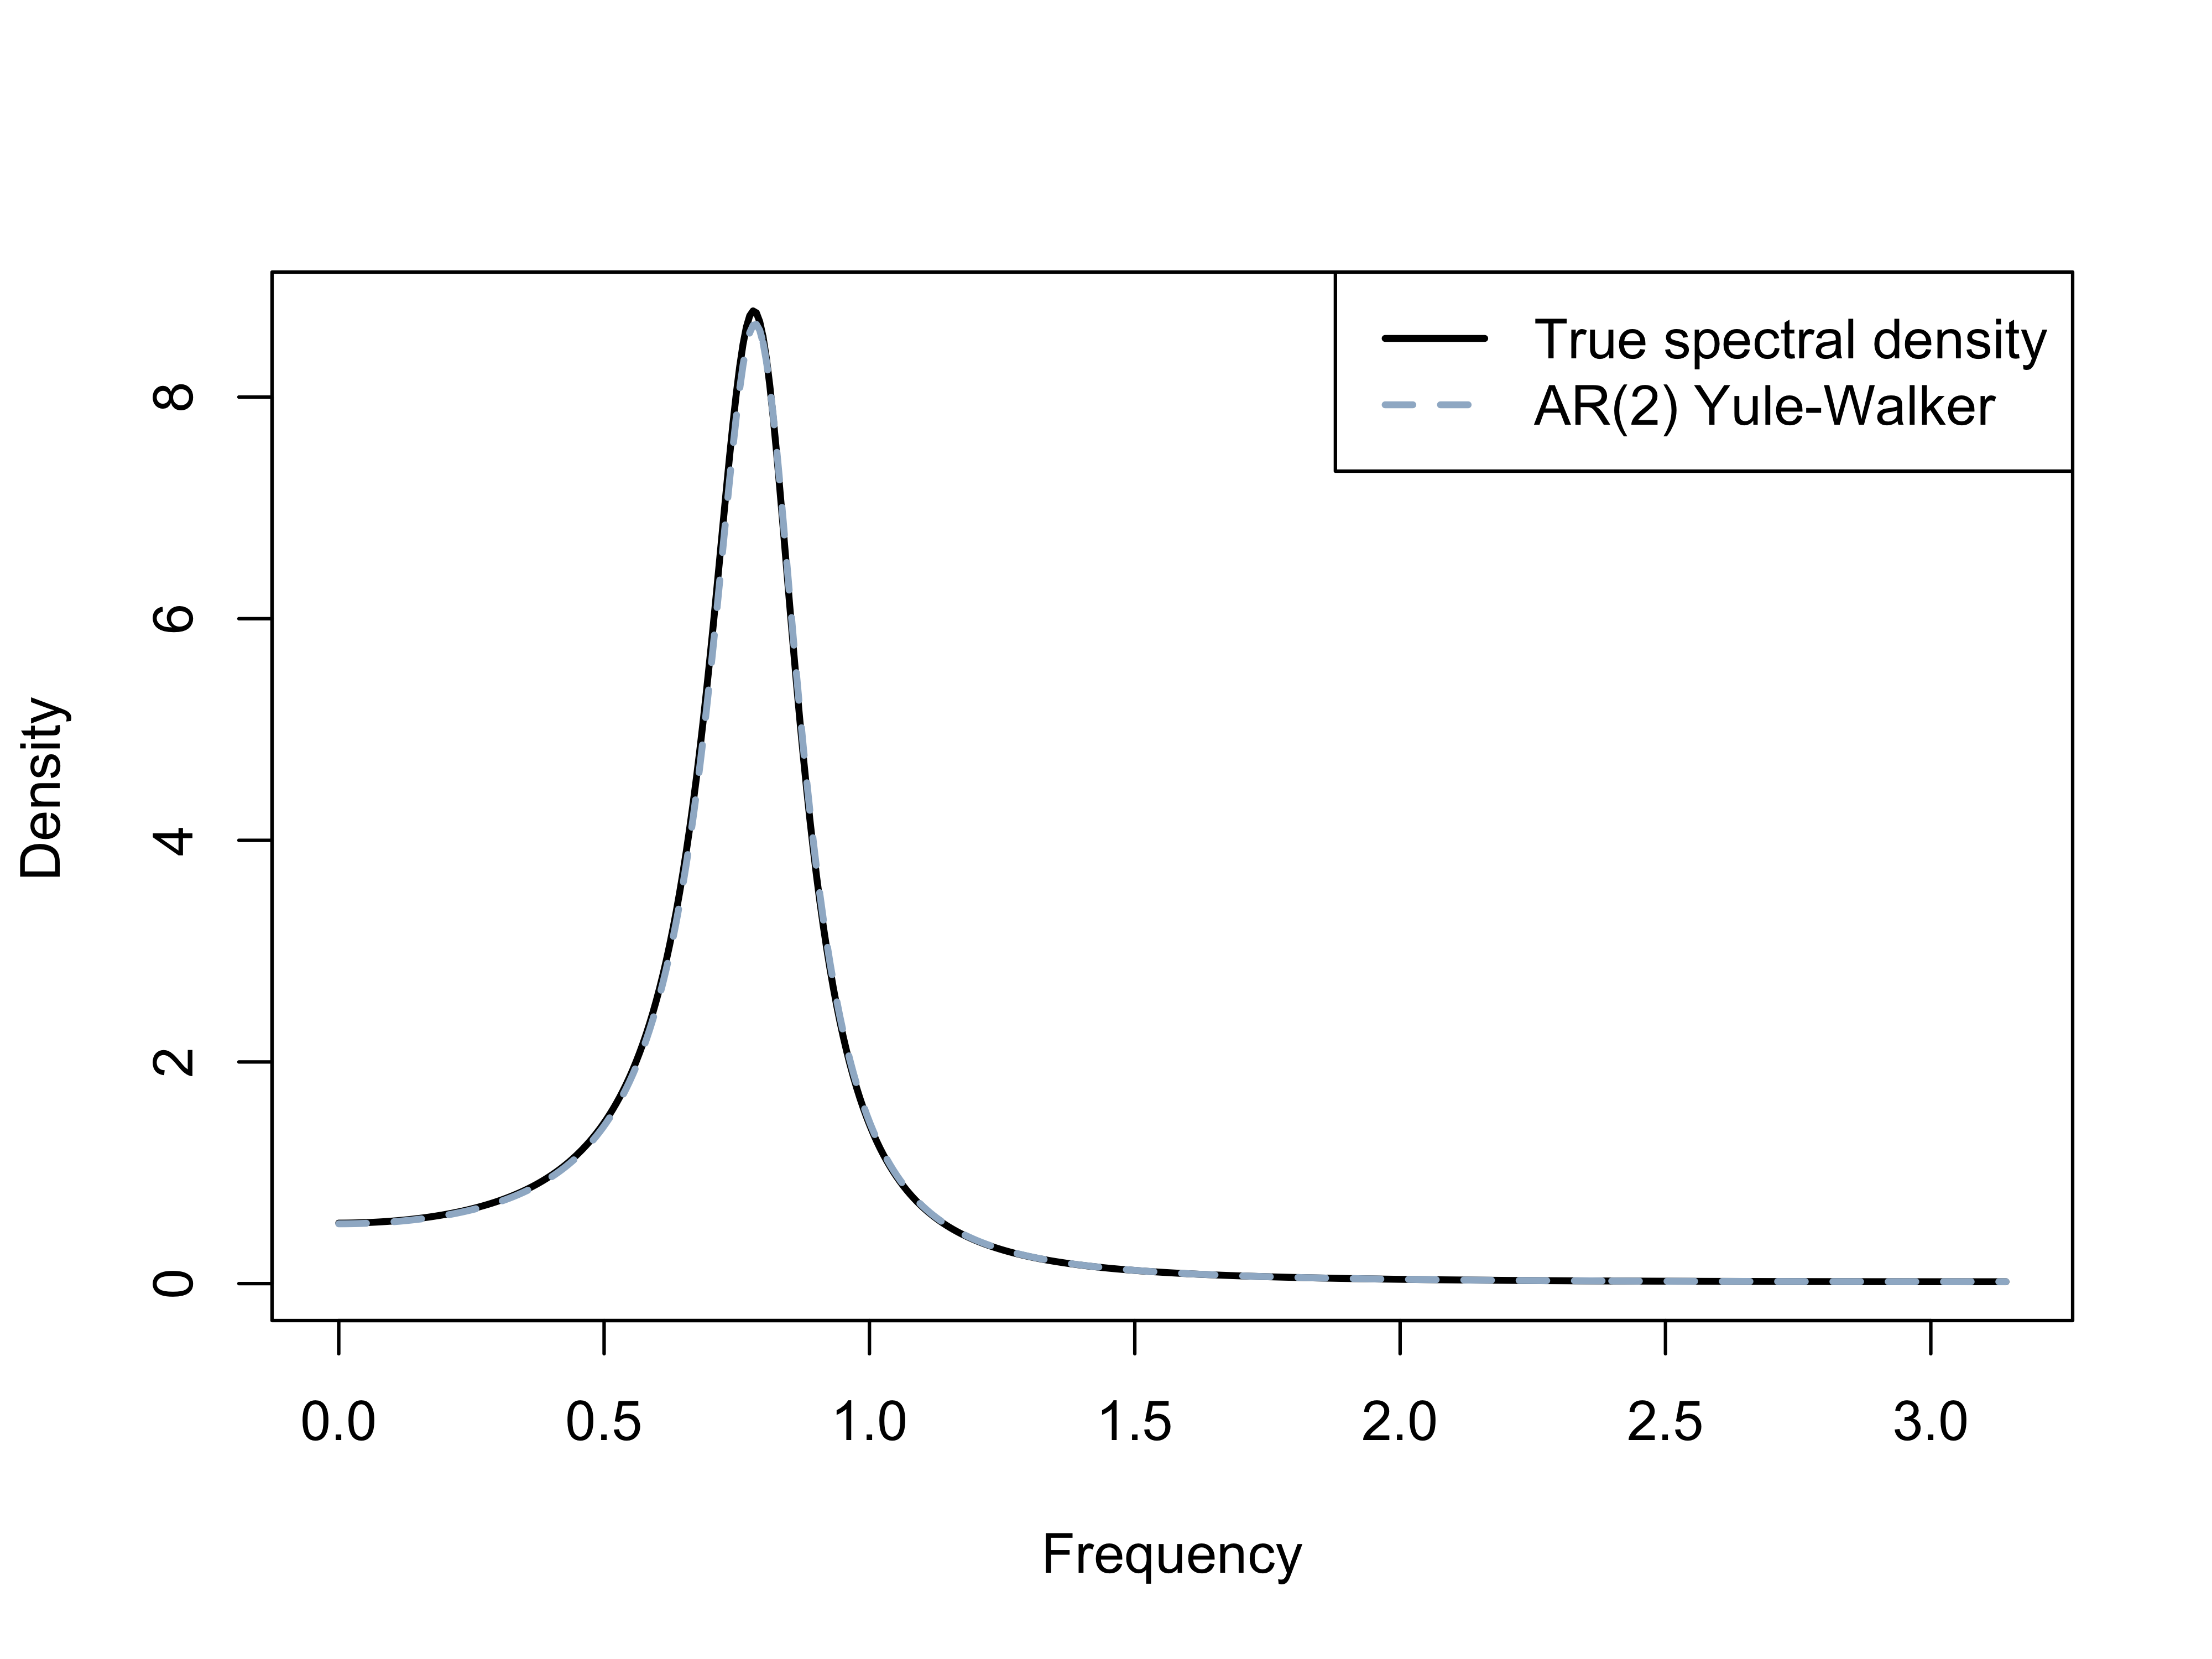
\includegraphics[width=0.8\linewidth]{ar2plot.png}
    \caption{\textbf{True Spectral Density and $AR(2)$ Spectral Density.} The estimated spectral density obtained from fitting $AR(2)$ model on the simulated process is visually close to the true spectral density.}
    \label{fig:ar2_vs_true}
\end{figure}

To assess the goodness--of--fit between the true spectral distribution and the one implied by the fitted AR(2) model, we implement the CvM test. This test quantifies the discrepency between two distribution functions by measuring the average squared distance between them. In our setting, we compare the empirical cumulative spectral distribution of the AR(2) estimator, $\widehat F_{AR}(\omega)$, with the true cumulative spectral distribution $F(\omega)$. The hypotheses are
\begin{equation}
    \begin{aligned}
        &H_0: \widehat F_{AR}(\omega) = F(\omega)\\
        &H_A: \widehat F_{AR}(\omega) \neq F(\omega)
    \end{aligned}
\end{equation}
The CvM test statistic is then defined as
\begin{equation}
    T_{\mathrm{CvM}} = \int_{\omega_{min}}^{\omega_{max}} (\widehat F_{AR}(\omega) - F(\omega) )^2d\omega.
\end{equation}
For spectral density testing, we cannot use the standard CvM critical values since it requires i.i.d observations, but our time series has temporal dependency. Therefore, we are going to generate the null distribution via bootstrap, which gives the distribution of the test statistics under the null hypothesis. For each bootstrap sample, we sample an AR(2) from the residuals of the fitted AR(2) model, which resembles white noise as seen in Figure \ref{fig:resid_distr}, and calculate the test statistics for each sample.
The p--value used is the proportion of observing the bootstrapped test statistics that is greater than the observed test statistics. Our study suggests a p--value $0.706$, which means that the estimated spectral density is consistent with the true spectral density at the significance level $\alpha=0.05$. 

\begin{figure}[ht!]
    \centering
    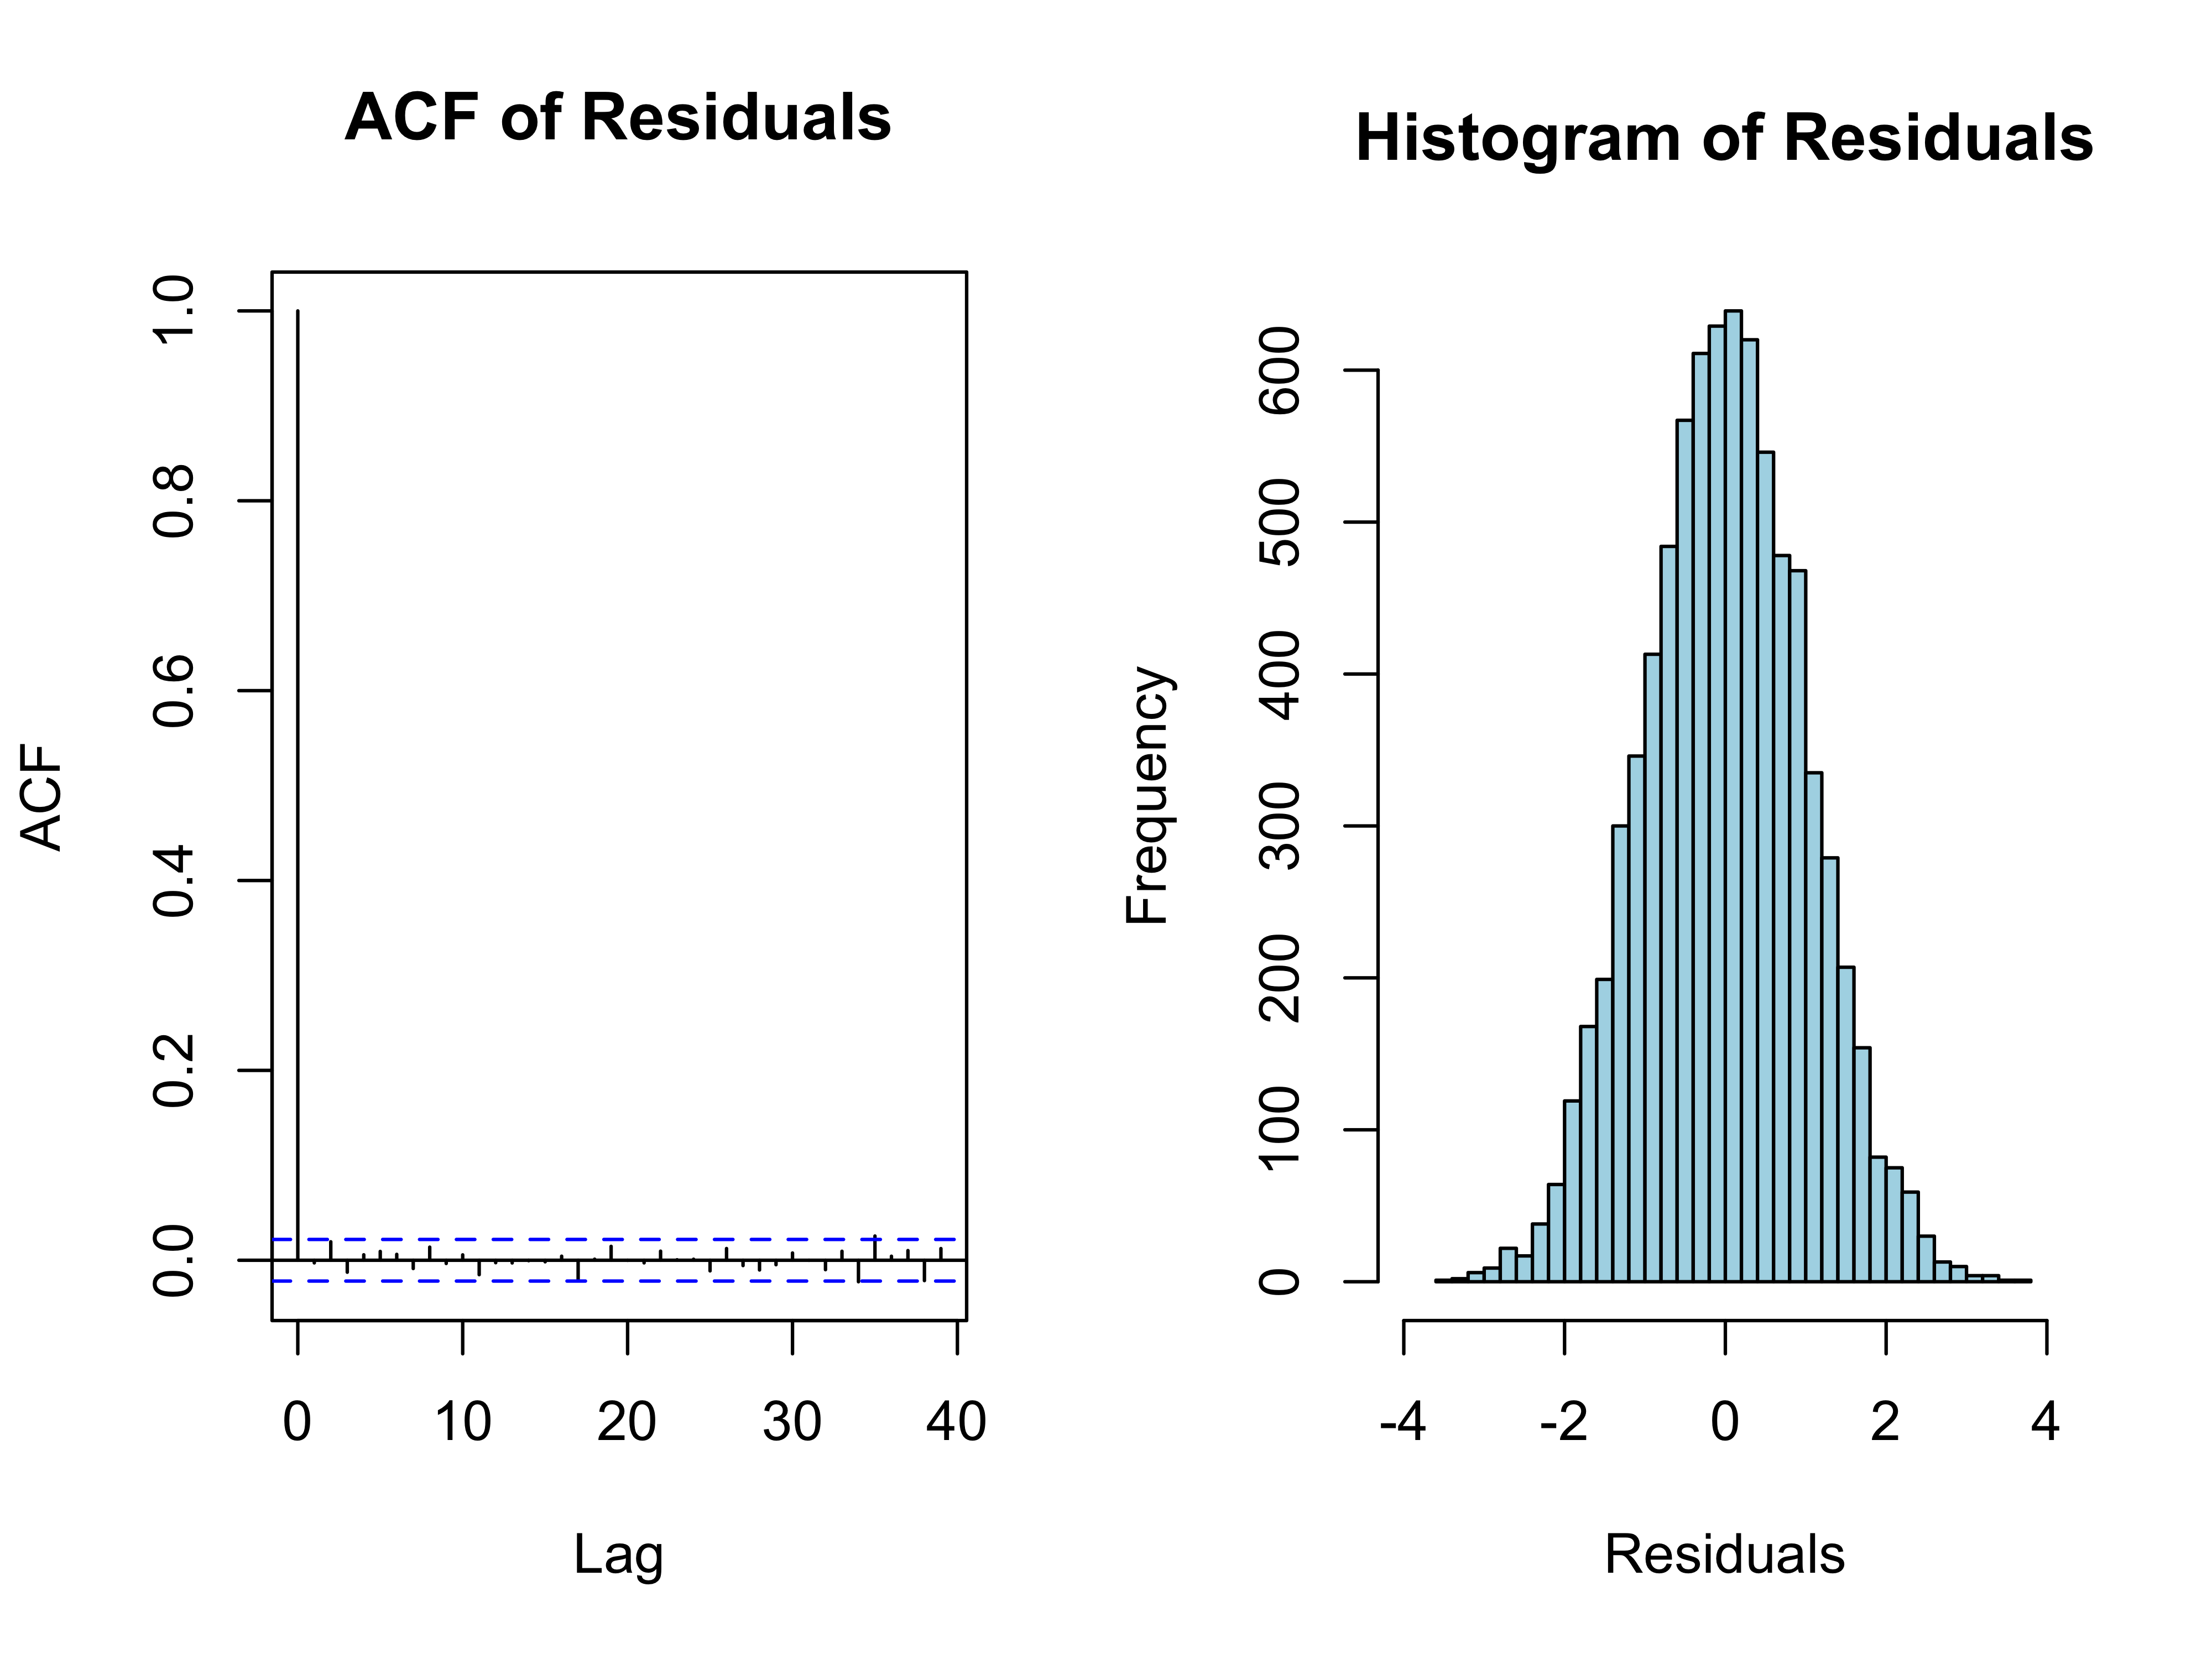
\includegraphics[width=0.8\linewidth]{ar_residuals.png}
    \caption{\textbf{Residuals of the $AR(2)$ model.} As observed from the ACF plot, the residuals seem to resemble white noise, and from the histogram, the residuals look normally distributed as well.}
    \label{fig:resid_distr}
\end{figure}

To assess the extent of model misspecification, we compute the KL divergence between each candidate model’s spectral density and the true spectral density of the data-generating process. Specifically, we evaluate $MA(q), AR(p) $ and $ARMA(p,q)$ models over a range of orders $(p,q)$ as potential approximating models for the underlying stationary process. Because the data--generating mechanism is a causal $AR(2)$, process—i.e., one whose autoregressive polynomial has all roots outside the unit circle—its spectral density admits an infinite--order moving average representation. Consequently, any finite--order $MA(q)$ with $q \leq 5$ cannot reproduce the true spectrum, and therefore exhibits a substantially larger KL divergence relative to the AR and ARMA models. Additionally, a lower order than the true order of the $AR$ model also performs poorly because it cannot reproduce the correct pattern of the spectral density due to having too few roots for the polynomial. This pattern is clearly reflected in Figure~\ref{fig:models_kl_error}, where all finite--order MA models display markedly higher divergence values. In contrast, any $ARMA(2,q)$ model performs comparably to the correctly specified $AR(2)$ model in estimating the spectral density of the underlying process, as the inclusion of additional moving--average terms does not alter the fundamental autoregressive structure that governs the spectrum. This reinforces the necessity of careful model identification (e.g., via a Box--Jenkins--type procedure) prior to estimating spectral quantities, as underspecified models can lead to significant distortions in the estimated spectrum.


\begin{figure}[ht!]
    \centering
    \includegraphics[width=0.8\linewidth]{kl_dvg_error_plot.png}
    \caption{\textbf{KL divergence across different models.} KL divergence between the true $AR(2)$ spectral density and various AR, MA, and ARMA models. Finite-order MA models and low order AR($p$) and $ARMA(p,1)$ ($p=1)$ models exhibit large divergence due to misspecification, whereas AR($p$) and $ARMA(p,q)$ with $p \geq 2$ models achieve near-zero divergence and successfully recover the underlying spectral structure. }
    \label{fig:models_kl_error}
\end{figure}


\subsection{Estimation of the Autocovariance Function (ACVF)}
In this section, we will explore techniques to estimate the stationary process $X_t$ without making a model assumption. Instead, we will estimate its ACVF $\widehat \Gamma(k)$ and its spectral density $\widehat F(\lambda)$. 
As suggested in \cite{brockwelldavis2016}, we use cross moment sampling to estimate the ACVF as follows: 
\begin{equation}\label{eq:hatgam}
    \widehat \Gamma_X(h) = \frac{1}{n} \sum_{t=1}^{n-|h|} (X_{t+|h|} - \overline X_n)(X_t - \overline X_n)
\end{equation}
where the moment estimator of the mean $\mu$ of a stationary process is the sample mean: \\ $\overline X = \frac{X_1 + ... +X_n}{n}$. 


Note that the estimator is biased, even if we scale it by $(n-h)^{-1}$ instead of $n^{-1}$. 
\begin{theorem}[Central Limit Theorem for a Stationary Process (Thm 7.1.2 in Davis \& Brockwell Time Series Theory and Methods)] \label{CLT}
    Let $\{X_t\}_{t=1}^T$ be a strictly stationary, zero-mean, linear process:
    $$X_t = \mu + \sum_{i=0}^\infty \psi_i Z_{t-j}$$\\
    where $\sum_{i=0}^\infty |\psi_i| < \infty, Z_t \sim IID(0,\sigma^2)$.\\
    Then:
    $$\overline X_n \sim \text{AN}(\mu, n^{-1} \nu)$$\\
    where $\nu = \sum_{h = -\infty} ^\infty \gamma(h) = \sigma^2 ( \sum_{i=0}^\infty \psi_i)^2$, and $\gamma(\cdot)$ is the autocovariance function of $\{X_t\}$.
\end{theorem}

WLOG, we assume that $\mathbb{E}[X_t] =0$ then we can simplify $\gamma(h)$ using Theorem~\ref{CLT}
\begin{equation}\label{eq:acvf_bias}
    \begin{aligned}
        \mathbb{E}[\widehat \Gamma_X(h)] &= \frac{1}{n} \sum_{t=1}^{n-|h|}\mathbb{E}\left[ X_{t+|h|} X_t + \bar{X_n}^2 \right ]\\
        & =  \frac{1}{n} \sum_{t=1}^{n-|h|} \gamma(h) + \mathbb{E}[\overline X_n^2]\\
        \text{Using Theorem} ~\ref{CLT}: &\sqrt{n}\,\overline X_n \xrightarrow{d} N(0,\nu),\text{ so that } \overline X_n = \mathcal{O}_p(n^{-1/2})\\
\mathbb{E}[\overline X_n^2] &= \operatorname{Var}(\overline X_n)
= \frac{\nu}{n} + \mathcal{O}\left(\frac{1}{n}\right).\\
\text{Therefore:}\\
       \mathbb{E}[\widehat \Gamma_X(h)] &= \left(1-\frac{|h|}{n} \right)\gamma(h) +\frac{\nu}{n} + \mathcal{O}\left(\frac{1}{n}\right)
    \end{aligned}
\end{equation}

This estimator is obviously biased, however, it becomes asymptotically unbiased as $n \rightarrow \infty$. We consider scaling the sampled cross moments with $n^{-1}$ since it guaranties that the $k$--dimensional sample covariance matrix ( $\widehat \Gamma_k$) is positive definite, which is the property we need to ensure that the estimated spectral density $\widehat F$ is a valid density. 
The $k$--dimensional sample covariance matrix is:
\begin{equation}
\label{eq:Gamma_k_toeplitz}
\hat{\Gamma}_k =
\begin{bmatrix}
\hat{\gamma}(0) & \hat{\gamma}(1) & \cdots & \hat{\gamma}(k-1) \\
\hat{\gamma}(1) & \hat{\gamma}(0) & \cdots & \hat{\gamma}(k-2) \\
\vdots          & \vdots          & \ddots & \vdots          \\
\hat{\gamma}(k-1) & \hat{\gamma}(k-2) & \cdots & \hat{\gamma}(0)
\end{bmatrix}
\end{equation}

We can rewrite $\widehat \Gamma_k$ as: 
\begin{equation}
\begin{aligned}
    \widehat \Gamma_k &= \frac{1}{n} C^TC
\end{aligned}
\end{equation}
Where C is an $n \times k $ matrix, in which each column represents the centered time series at different lags:
$$C = \begin{bmatrix}
X_1 - \bar{X} & X_2 - \bar{X} & X_3 - \bar{X} & \cdots & X_k - \bar{X} \\
X_2 - \bar{X} & X_3 - \bar{X} & X_4 - \bar{X} & \cdots & X_{k+1} - \bar{X} \\
X_3 - \bar{X} & X_4 - \bar{X} & X_5 - \bar{X} & \cdots & X_{k+2} - \bar{X} \\
\vdots & \vdots & \vdots & \ddots & \vdots \\
X_{n-k+1} - \bar{X} & X_{n-k+2} - \bar{X} & X_{n-k+3} - \bar{X} & \cdots & X_n - \bar{X}
\end{bmatrix}$$

In which we can see that
\begin{equation}
    \begin{aligned}
        a^T \widehat \Gamma_k a &= a^T \frac{1}{n}C^T C a\\
        &= \frac{1}{n} (a^T C^T)(Ca) \\
        &= ||Ca||^2 \geq 0
    \end{aligned}
\end{equation}
Therefore, the estimate $\widehat \Gamma(k)$ from the Eqn.~\ref{eq:hatgam} is positive definite, hence by Theorem ACVF it is an autocovariance function, and the spectral density is the spectral distribution of both $\gamma(k)$ and the stationary process $\{X_t\}$. \\
When we scale by $(n-|k|)^{-1}$, not all lags are given equal weight, and the larger lags are given more weight, that is, $\tilde \gamma (k-1) = \frac{1}{n-k+1} \sum_{t=1}^{n-k+1} (X_t - \overline X)(X_{t+k-1} - \overline X)$. Hence, each element has a different denominator, so we cannot rewrite the matrix $\widehat \Gamma_k$ as $D^TD$ for some matrix $D$. Therefore, $\widehat \Gamma_k$ might not be positive definite.

\subsection{Estimation of the Spectral Density}

Given the estimated ACVF $\{\widehat \Gamma(h)\}_{h=-(n-1)}^{n-1}$, there are several ways to construct
an estimator $\widehat F(\omega)$ of the spectral density. In this paper we
focus on two broad classes: (i) estimators obtained by (finite) Fourier
transforms of the estimated ACVF, and (ii) smoothed or lag--window type
estimators. For each method, we will study its consistency.

\subsubsection{Estimation of Spectral Density using Discrete Fourier Transform of Circulant Matrices}
A natural ACVF--based estimator of the spectral density is the finite Fourier
transform
\begin{equation}
    \begin{aligned}
        \widehat F(\omega) &= \frac{1}{2 \pi} \sum_{h = -(n-1)}^{n-1} \widehat \Gamma(h) e^{-i h \omega}\\
    \end{aligned}
\end{equation}

The empirical covariance matrix  $\widehat \Gamma_n = \{\widehat \Gamma(j-k)\}_{j,k=1}^n$ has a Toeplitz structure.
For large $n$ it is common to approximate this Toeplitz matrix by a circulant
matrix whose first row is constructed from the ACVF. Circulant matrices are
diagonalized by the discrete Fourier transform (DFT), so their eigenvalues
are obtained by applying the DFT to the first row. This provides an
efficient $O(n \log n)$ implementation, via the fast Fourier transform
(FFT), both for evaluating spectral estimates on a frequency grid and
for performing large--scale covariance computations based on $\widehat \Gamma_n$.

We start by constructing a circulant matrix $C_n$ from the Toeplitz matrix in Eqn.~\ref{eq:Gamma_k_toeplitz}, where $\sigma_0 = \widehat \Gamma(0), \sigma_{h} = \widehat \Gamma(h), 1 \leq h \leq n-1$:
\begin{equation}
    [C_n]_{ij} = \sigma_{(i-j)\text{(mod n)}}
\end{equation}

Because the modular index satisfies
\begin{equation}
    (i-j) \text{ mod }n = \begin{cases}
        h \quad \text{ equivalent to lag } +h\\
        n-h \quad  \text{ equivalent to lag } -h
    \end{cases}
\end{equation}
Since the process is stationary $\gamma(h) = \gamma(-h)$, we can still use $\sigma_h = \widehat \Gamma(h)$.

Therefore, we can safely define that the generator $\sigma$ as follows:
\begin{equation}
    \begin{aligned}
        \sigma_0 &= \widehat \Gamma(0)\\
        \sigma_h &= \hat{\gamma(h)}, \quad h = 1,...,n-1\\
        \sigma_{n-h} &= \hat{\gamma(-h)}, \quad h = 1,...,n-1\\
    \end{aligned}
\end{equation}

We can show that the Frobenius norm of the difference between the circulant matrix $C_n$ and the ACVF matrix $\widehat \Gamma_n$ converges to 0 as $n  \to \infty$:
\begin{equation}
    \lim_{n\to \infty} \frac{1}{n^2} ||\widehat \Gamma_n - C_n||^2_F = 0 
\end{equation}
The proof is covered in Prof. Peters Lecture Notes.

The circulant matrix $C_n \in \mathbb{C}^{n\times n}$ admits the spectral decomposition:
\begin{equation}\label{eq:circulant_decomp}
    C_n = F^{-1}\Lambda F,
\end{equation}
where $F$ denotes the $n\times n$ discrete Fourier transform (DFT) matrix
with entries 
\begin{equation}
    F_{jk} = \exp\!\left(-\frac{2\pi i}{n} jk \right),\qquad j,k=0,\dots,n-1.
\end{equation}
The matrix $\Lambda = \operatorname{diag}(\lambda_0,\dots,\lambda_{n-1})$
is diagonal and contains the eigenvalues of $C$, given explicitly by the
DFT of its first column:
\begin{equation}
    \lambda_k = \sum_{h=0}^{n-1} \sigma_h \exp\!\left(-\frac{2\pi i}{n} hk \right),
    \qquad k=0,\dots,n-1,
\end{equation}
where $(\sigma_0,\dots,\sigma_{n-1})$ is the generating vector of the circulant matrix.  
Thus, the factorization $C = F^{-1}\Lambda F$ expresses the fact that every circulant matrix is unitarily diagonalized by the Fourier basis. 
Therefore, the spectral density embedded at the Fourier frequencies is:

\begin{equation}
\begin{aligned}
     \widehat F_{\text{circ}}(\omega_k) &= \frac{1}{2\pi}\lambda_k \\
     &= \frac{1}{2\pi} \left( \widehat \Gamma(0) + \sum_{h=1}^{n-1} \hat\gamma(h)e^{-ih\omega_k} +  \sum_{h=1}^{n-1} \hat\gamma(-h)e^{-i(-h)\omega_k} \right)\\
     &=  \frac{1}{2\pi} \left( \widehat \Gamma(0) + \sum_{h=1}^{n-1} \hat\gamma(h)e^{-ih\omega_k} + \sum_{h=-(n-1)}^{-1}  \hat\gamma(h)e^{-i(h)\omega_k}\right)\\
     &=  \frac{1}{2\pi}  \sum_{h=-(n-1)}^{n-1} \hat\gamma(h)e^{-ih\omega_k},
\quad \omega_k = \frac{2 \pi k}{n}
\end{aligned}
\end{equation}
To check for biasness, we compute the first moment of the estimator $\widehat F_{\text{circ}}(\omega_k)$. 
\begin{equation}
    \begin{aligned}
        \mathbb{E} [\widehat F_{circ} (\omega_k)] = \frac{1}{2\pi}  \sum_{h=-(n-1)}^{n-1} \mathbb{E}\left[ \widehat \Gamma(h)\right]e^{-ih\omega_k}
    \end{aligned}
\end{equation}

This estimator is asymptotically unbiased because from  Eqn.~\ref{eq:acvf_bias}, we can see that $\widehat \Gamma(h)$ is asymptotically unbiased. 

However, this estimator is inconsistent. Therefore, we will show another way to estimate the spectral density using Welch's method, which is an average of successive blocks of periodogram over time. This method will reduce the variance of the raw periodogram above. 

\subsubsection{Welch's Method for Spectral Density Estimation}
\noindent{\bf Estimation Procedure} \\
We begin with a stationary time series data $\{ X_t\}_{t=1}^T$, which is truncated into $K$ segments, each of length $L$. This truncation is equivalent to using a rectangle window, which creates artificial discontinuities at the boundaries. This window has the form (\cite{brockwelldavis2016}):

\begin{equation}
w(t) = 
    \begin{cases}
        1 \quad \text{ if } |x| \leq 1 \\
        0 \quad\text{otherwise}
    \end{cases}
\end{equation}
and the spectral window (the normalized squared Fourier transform of the taper) is given by the Dirichlet kernel:
\begin{equation}\label{eq:w_rect}
    W_{rect}(\omega) \propto \frac{1}{2 \pi} \frac{\sin((r+\frac{1}{2})\omega)}{\sin(\omega/2)}, \quad r = \frac{L-1}{2}
\end{equation}

With this window, $W(\omega)$ is negative at certain $\omega$, which leads to a negative estimate of the spectral density at some frequencies $\omega$. To mitigate this, we introduce multiple windows: Barlett, Hanning and Blackman, which are covered in \cite{harris1978}.
Our series has a general form:
\begin{equation}
    Y_t^{(k)} = w(t) X_t^{(k)}
\end{equation}

All taper windows reduce the weights at the segment endpoints, with $w(0) \approx 0 \text{ and } w(L-1)\approx 0$. Therefore, to avoid loss of information, we are going to truncate the stationary series into overlapping segments. The overlap portions ensure that observations near the boundary of one block appear near the center of another, where the taper weights are close to 1. It is controlled by the shift $D$, which for 50\% overlap, $D=L/2$. If the shift is $D$, then the $k-th$ segment is
\begin{equation}
    X_t^{(k)} = X_{t+(k-1)D}
\end{equation}
Using the taper windows, the series is now defined as
\begin{equation}
    Y_t^{(k)} = w(t) X_t^{(k)}
\end{equation}
where $w(t)$ represents the time--domain taper window. 

We then proceed to compute the tapered periodogram of each segment using the window-power normalization, which is taper window specific. 
\begin{equation}\label{eq:tapered_periodogram}
    I_k(\omega)= \frac{1}{2\pi L\,U_w} \left|\sum_{t=0}^{L-1}Y^{(k)}_t\, e^{-i \omega t}\right|^2,
\end{equation}
where
\begin{equation}
    \label{eq:window_power}
    U_w = \frac{1}{L} \sum_{t=0}^{L-1} w(t)^2
\end{equation}
is the window--power normalization constant, ensuring that the estimator
is correctly scaled. 

The Welch spectral density estimator is obtained by averaging the tapered periodograms over all $K$ segments:
\begin{equation}
    \label{eq:welch_estimator}
    \widehat{f}_{\mathrm{Welch}}(\omega)
    =
    \frac{1}{K} \sum_{k=1}^K I_k(\omega).
\end{equation}

Taper windows like Hanning and Blackman can be written as linear combinations of cosines, and cosines correspond to frequency shifts. Therefore, their spectral windows can be written as weighted combinations of shifted rectangular spectral windows from  Eqn.~\ref{eq:w_rect}. The Barlett window is constructed as a triangular, not a combination of cosines, hence it is the convolution of two rectangular windows. These spectral windows $W(\omega)$ will be used later to compare the speed of convergence to the true $f(\omega)$, since even though the estimates using these taper windows are consistent, they are biased. 
\noindent{\bf Hanning (Hann) Window.}
\begin{equation}
    \begin{aligned}
        w(t) &= 0.5\left(1-\cos\left( \frac{2\pi t}{L-1}\right)\right), \quad t=1,\dots,L-1\\
        W_{\mathrm{Hann}}(\omega)&=
\frac{1}{2}W_{\mathrm{rect}}(\omega)
-\frac{1}{4}W_{\mathrm{rect}}(\omega + \tfrac{2\pi}{L-1})
-\frac{1}{4}W_{\mathrm{rect}}(\omega - \tfrac{2\pi}{L-1})\\
    \end{aligned}
\end{equation}
where $W_{rect}(\omega)$ is the rectangle spectral window from  Eqn.~\ref{eq:w_rect}.

\noindent{\bf Blackman Window.}

\begin{equation}
    \begin{aligned}
        w_{\mathrm{Blackman}}(t) &=0.42 - 0.5\cos\left(\frac{2\pi t}{L-1}\right) + 0.08\cos\left(\frac{4\pi t}{L-1}\right), \qquad t = 0,\dots,L-1.\\
        W_{\mathrm{Blackman}}(\omega)&=0.42\, W_{\mathrm{rect}}(\omega)- 0.25\, W_{\mathrm{rect}}\!\left(\omega + \tfrac{2\pi}{L-1}\right)
- 0.25\, W_{\mathrm{rect}}\!\left(\omega - \tfrac{2\pi}{L-1}\right) \\[4pt]
&\quad
+ 0.04\, W_{\mathrm{rect}}\!\left(\omega + \tfrac{4\pi}{L-1}\right)
+ 0.04\, W_{\mathrm{rect}}\!\left(\omega - \tfrac{4\pi}{L-1}\right)
    \end{aligned}
\end{equation}

\noindent{\bf Bartlett Window.}

\begin{equation}
\begin{aligned}
    w_{\mathrm{Bartlett}}(t)= (w_{rect} * w_{rect})(t)&= 
\begin{cases}
\dfrac{2t}{L-1}, & 0 \le t \le \dfrac{L-1}{2},\\[6pt]
2 - \dfrac{2t}{L-1}, & \dfrac{L-1}{2} \le t \le L-1.
\end{cases}\\
W_{\mathrm{Bartlett}}(\omega) = \big| W_{rect}(\omega)\big|^2 &= \left(\frac{\sin(\omega L/2)}{\sin(\omega/2)}\right)^2\\
\end{aligned}
\end{equation}

\subsection{Simulation Study: Spectral Density Estimation via Welch’s Method}
To illustrate the nonparametric procedure, we implement Welch’s method using Bartlett, Hanning and Blackman windows across different segment lengths $L \in \{256, 512, 1024\}$. We first apply the taper to each truncated segment. For each choice of window and segment length, we first estimate the sample autocovariance function for the truncated segments and then compute the corresponding windowed periodograms—i.e., the discrete Fourier transforms of the tapered ACVF estimates—using the appropriate normalization constant $U_w$. The Welch spectral estimate $\widehat F_{Welch}$ is obtained by averaging these windowed periodograms across all segments. Figure \ref{fig:compare_window_plot} provides a visual comparison of these window-based estimators against the true spectral density, allowing us to assess how window choice and segment length affect the quality and smoothness of the estimates.

\begin{figure}[!ht]
  \centering
  \includegraphics[width=150mm]{compare_window_plot.png} 
  \caption{\textbf{Comparison of Spectral Density Estimates.}
  This figure displays the estimated spectral densities using 3 different taper windows across 3 
  segment lengths (L = 256, 512, 1024). The shorter segments appear smoother, and the three windows 
  produce similar estimates.}
  \label{fig:compare_window_plot}
\end{figure}


We assess estimation accuracy using the KL divergence, which quantifies the difference between the estimated spectral density and the true density by calculating the expected log-likelihood loss when estimating. We choose to use KL divergence since it penalizes for deviations in both shape and magnitude of the spectrum. By computing the KL divergence for all combinations of taper windows and segment lengths, we identify the window–length configuration that provides the closest nonparametric approximation to the true spectrum.

% Table created by stargazer v.5.2.3 by Marek Hlavac, Social Policy Institute. E-mail: marek.hlavac at gmail.com
% Date and time: Sun, Nov 23, 2025 - 12:55:37

% \begin{table}[!htbp] \centering 
%   \caption{This table displays the Integrated Squared Error (ISE) of each of the taper window method with various segment length and the true spectral density found from our simulation study. Based on this result, Hanning window with length 256 seems to be outperforming all other windows and lengths.} 
%   \label{window_comp_wise} 
% \begin{tabular}{@{\extracolsep{5pt}} cccc} 
% \\[-1.8ex]\hline 
% \hline \\[-1.8ex] 
% Segment Length & Hann &Bartlett & Blackman\\
% 256 & $0.149$ & $0.150$ & $0.169$ \\ 
% 512 & $0.233$ & $0.233$ & $0.250$  \\ 
% 1024 &$0.437$ & $0.461$ & $0.460$ \\ 
% \hline \\[-1.8ex] 
% \end{tabular} 
% \end{table} 

 
\begin{equation}
    D_{KL}(f|| \widehat F) \approx \sum_{k=1}^Kf(\omega_k) \log \left(\frac{f(\omega_k)}{\widehat F(\omega_k)} \right ) \Delta \omega.
\end{equation}
Our result in Table \ref{window_comp_kl} indicates that the Hanning window with segment length 256 yields the closest estimated spectral density. 

\begin{table}[!htbp] \centering 
  \caption{This table displays the KL divergence of each of the taper window method with various segment length and the true spectral density found from our simulation study. Based on this result, Hanning window with length 256 seems to be outperforming all other windows and lengths.} 
  \label{window_comp_kl} 
\begin{tabular}{@{\extracolsep{5pt}} l|ccc} 
\\[-1.8ex]\hline 
\hline \\[-1.8ex] 
Segment Length & Hann &Bartlett & Blackman\\
256 &$0.056$ & $0.067$ & $0.059$ \\ 
512 & $0.085$ & $0.092$ & $0.093$  \\ 
1024 & $0.121$ & $0.122$ & $0.121$ \\ 
\hline \\[-1.8ex] 
\end{tabular} 
\end{table} 

\noindent{\bf Hypothesis Test}

We conduct this hypothesis test to assess whether the estimated spectral density is statistically consistent with the true spectral density implied by the underlying AR(2) model.
The classical one-sample Kolmogorov–Smirnov (KS) test compares an empirical CDF with a fully specified theoretical CDF. 
\begin{equation}
    \begin{aligned}
        H_0&: \widehat F(\omega) =  F(\omega)\\
        H_A&: \widehat F(\omega) \neq  F(\omega)
    \end{aligned}
\end{equation}

Under the assumption that the $n$ observations are i.i.d., the KS statistic is:
\begin{equation}
    \begin{aligned}
        D= \sup_x |F_n(x)- F(x)|
    \end{aligned}
\end{equation}
which has a known Kolmogorov distribution, from which standard critical values and p--values are derived.

However, this theoretical justification relies on i.i.d. observations and the classical empirical--CDF framework. Because the KS test assumes i.i.d. data and a classical empirical--CDF setting, the standard Kolmogorov critical values are not valid for our spectral--density comparison problem due to correlation in temporal data. Consequently, the sampling distribution of the KS-type statistic is unknown.
To obtain a valid test, we employ a bootstrap procedure under the null model. We generate new time-series replicates by sampling the (approximately Gaussian) residuals and reconstructing a stationary $AR(2)$ process that would have arisen if the null hypothesis were true, thereby preserving the temporal dependence structure. For each bootstrap sample $b$, we apply the same Welch estimation pipeline, compute the corresponding spectral CDF $\widehat F^{(b)}(\omega) = \int_0^\omega \widehat F_{Welch}(\lambda)^{(b)}d\lambda$, and calculate the KS-type statistic $D^{(b)} = \sup_{\omega} |\widehat F^{(b)}(\omega)- F(\omega)|$ for each bootstrap sample. The collection ${D^{(b)}}_{b=1}^B$ provides an empirical approximation to the null distribution of the test statistic. The bootstrap p--value given by the proportion of bootstrap statistics exceeding the observed statistic correctly accounts for temporal dependence as well as all transformations involved in spectral estimation, yielding a valid test for equality of spectral densities:
\begin{equation}
    \hat p = \frac{1}{B}\sum_{b=1}^B \mathbbm{1}_{D^{(b)} > D_{obs}}, \quad 
\end{equation}

where $B$ is the number of bootstrap samples, $D^{(b)}$ is the KS test statistic of that bootstrap sample and $D_{obs}$ is the observed test statistics. 

Based on the results from Table \ref{window_comp_kl}, we conduct the hypothesis test for the spectral density computed using Hanning taper window with length $L=256$. 

The observed KS test statistics between the estimated spectral distribution $\widehat F(\omega)$ and the true spectral distribution $F(\omega)$ is $D_{\mathrm{obs}} = 0.017887.$

Under the null hypothesis $H_0$, we simulate data from the AR(2) model with parameters $\phi = (1.27,\,-0.81),\sigma = 1,$
and compute the KS--type statistic for each bootstrap replication.  This yields the empirical null distribution of $D$.
We obtain the bootstrap p--value 
\begin{equation}
    \hat p  =  \mathbb{P} (D^{(b)} \ge D_{\mathrm{obs}} \mid H_0) = 0.584.
\end{equation}
Thus, if $H_0$ is true, there is a $58.2\%$ chance of obtaining a value of $D$ at least as large as the observed statistic.
At significance level $\alpha = 0.05$, we have $\hat p = 0.582 \; \ge \; 0.05,$ therefore we fail to reject the null hypothesis.  
This indicates that the estimated spectral density is consistent with the true spectral density and that the estimation procedure produces reasonable results.


\section{Conclusion}
This report has investigated both parametric and nonparametric approaches to spectral density estimation through theoretical development and comprehensive simulation studies. Our investigation establishes the fundamental approximation theorem demonstrating that any stationary process spectral density can be arbitrarily closely approximated by an AR($p$) spectral density under appropriate conditions.
The parametric approach, examined through an AR(2) model specification, demonstrates strong performance when the model structure aligns with the underlying data-generating process. The CvM goodness--of--fit test fails to reject the null hypothesis of distributional equivalence between the theoretical and empirical spectral distribution functions, confirming that the correctly specified parametric model provides an efficient and parsimonious representation of the spectral characteristics. However, our model misspecification analysis reveals the critical vulnerability of parametric methods: models employing incorrect functional forms, such as imposing MA structure when the true process follows an AR specification, or insufficient model orders results in larger KL divergence. This consequence stems from the fundamental constraint that underspecified or misspecified parametric models lack the structural flexibility to accurately reconstruct complex spectral densities.
In contrast, the nonparametric approach demonstrates robustness to model uncertainty. While the initial circulant matrix implementation proved inconsistent for direct spectral density estimation, Welch's method improves the estimates without imposing restrictive parametric assumptions. The KS test corroborates the reliability of this optimally-tuned nonparametric estimator, demonstrating its ability to capture features of the spectrum that simpler parametric models may fail to reproduce.
These complementary findings shed light on the fundamental trade-off governing spectral density estimation methodology. Parametric methods tend to produce better results than classical nonparametric methods when the data length is relatively short but are subject to error from model misspecification. When the true spectral density exhibits complex structure—involving multiple peaks, irregular patterns, or features not readily captured by low--order AR or ARMA models—parametric approaches often fail to provide adequate approximations, regardless of estimation precision. Conversely, nonparametric methods may exhibit lower efficiency under correct parametric specification, yet they provide essential robustness when the true spectrum is too complex for low--order parametric models to capture. This robustness proves particularly valuable in exploratory analysis or applications where prior knowledge of the spectral structure is limited or unreliable. For example, macroeconomics times series often has structural breaks that violates the assumptions of the parametric models, in this case, nonparametric methods provide estimates without requiring the data to conform to a specific theoretical model. An interesting direction for future work is to explore the semiparametric spectral estimators, such as the local Whittle or hybrid AR–nonparametric smoothing methods, which combine the structural interpretability of parametric models with the flexibility of nonparametric estimators. Such approaches may offer improved robustness in settings where the spectrum exhibits both smooth long-run features and localized irregularities that are not well captured by either method alone.



\newpage

\section{Appendix}
For the choice of $\delta$ in the proof:
From Eqn.~\ref{eq:ar_prox_3}, we want to restrict the bound such that $\frac{\delta}{|XY|}$ does not get too large, which means we want $|XY|$ to not get too small, therefore we will find the lower bound for it. 
Since we have $Y > \frac{1}{M}$, and $X >  \frac{1}{M} - \delta$, we can consider the choice of $\delta$ to be at most $\frac{1}{2M}$. 

Additionally, with the $\epsilon$--$\delta$ style proof, we want
\begin{equation}\label{eq:eps_condition}
\left| \frac{1}{X} - \frac{1}{Y} \right| \leq \frac{\epsilon}{2}.
\end{equation}

From Eqn.~\ref{eq:ar_prox_3}, we also have
\begin{equation}\label{eq:delta_condition}
\left| \frac{1}{X} - \frac{1}{Y} \right| \leq \frac{\delta}{|XY|}.
\end{equation}

Therefore, to satisfy Eqn.~\ref{eq:eps_condition}, we must choose $\delta$ such that
\begin{equation}\label{eq:choose_delta}
\frac{\delta}{|XY|} \leq \frac{\epsilon}{2}
\quad \Longleftrightarrow \quad
\delta \leq \frac{\epsilon}{2} |XY|
\end{equation}
From Eqn.~\ref{eq:xy_bound}
\begin{equation}
|XY| > \frac{1}{2M^2},
\end{equation}
it follows that
\begin{equation}\label{eq:final_delta}
\frac{\epsilon}{2}|XY| \geq \frac{\epsilon}{4M^2}
\end{equation}

Therefore, combining with the condition that $\delta \geq \frac{1}{2M}$, we choose 
$$\delta = \min \left( \frac{1}{2M}, \frac{\epsilon}{4M^2} \right)$$
 to guarantee that :
\begin{equation}
\big| [A|\phi(e^{-i\lambda})|^2]^{-1} - f_p(\lambda) \big|  \leq \frac{\epsilon}{2}.
\end{equation}



% \begin{figure}[!ht]
%   \centering
%   \includegraphics[width=150mm]{}
%   \caption{}
%   \label{}
% \end{figure}

% \begin{table}[!ht]
% \centering
% \caption{}
% \begin{tabular}{}
% \hline
% \\
% \hline
% \end{tabular}
% \label{}
% \end{table}

\newpage

\begin{thebibliography}

\bibitem[Brockwell and Davis (2016)]{brockwelldavis2016}
Brockwell, Peter J. and Davis, Richard A. 
\newblock \textit{Introduction to Time Series and Forecasting}, 3rd edition. 
\newblock Springer Texts in Statistics. 
\newblock Springer, Cham, 2016. 
\newblock ISBN: 978-3-319-29852-8 (Hardcover), 978-3-319-29854-2 (eBook). 
\newblock \href{https://doi.org/10.1007/978-3-319-29854-2}{https://doi.org/10.1007/978-3-319-29854-2}.

\bibitem[Choudhuri et al (2004)]{choudetal}
Choudhuri, Nidhan, et al. 
\newblock ``Bayesian Estimation of the Spectral Density of a Time Series.''
\newblock \textit{Journal of the American Statistical Association}, vol. 99, no. 468, 2004, pp. 1050–59.
\newblock \href{http://www.jstor.org/stable/27590484}{http://www.jstor.org/stable/27590484}. 

\bibitem[Granger and Joyeux (1980)]{granger}
Granger, C.W.J. and Joyeux, R. 
\newblock ``AN INTRODUCTION TO LONG-MEMORY TIME SERIES MODELS AND FRACTIONAL DIFFERENCING.''
\newblock \textit{Journal of Time Series Analysis}, 1: 15-29.
\newblock \href{https://doi.org/10.1111/j.1467-9892.1980.tb00297.x}{https://doi.org/10.1111/j.1467-9892.1980.tb00297.x}. 

\bibitem[Harris (1978)]{harris1978}
Harris, F. J. 
\newblock ``On the use of windows for harmonic analysis with the discrete Fourier transform." 
\newblock \textit{Proceedings of the IEEE}, vol.~66, no.~1, pp.~51--83, Jan.~1978. 
\newblock \href{https://doi.org/10.1109/PROC.1978.10837}{https://doi.org/10.1109/PROC.1978.10837}. 

\bibitem[Harvey and Trimbur (2003)]{harvey}
Harvey, Andrew C., and Thomas M. Trimbur.
\newblock ``General Model-Based Filters for Extracting Cycles and Trends in Economic Time Series." 
\newblock \textit{The Review of Economics and Statistics}, vol. 85, no. 2, 2003, pp. 244–55.
\newblock \href{https://www.jstor.org/stable/3211576}{https://www.jstor.org/stable/3211576}. 



\bibitem[Wahba (1980)]{wahba}
Wahba, Grace
\newblock ``Automatic Smoothing of the Log Periodogram.''
\newblock \textit{Journal of the American Statistical Association}, Volume 75, Issue 369 (Mar., 1980),
122-132.
\newblock \href{https://doi.org/10.2307/2287399}{https://doi.org/10.2307/2287399}

\bibitem[Welch (1967)]{welch1967}
Welch, P.
\newblock ``The use of fast Fourier transform for the estimation of power spectra: A method based on time averaging over short, modified periodograms."
\newblock \textit{IEEE Transactions on Audio and Electroacoustics}, vol.~15, no.~2, pp.~70--73, June~1967.
\newblock \href{https://doi.org/10.1109/TAU.1967.1161901}{https://doi.org/10.1109/TAU.1967.1161901}.


\end{thebibliography}



\end{document}
